\documentclass[times, utf8, diplomski]{fer}
\usepackage{booktabs}
\usepackage[croatian]{babel}
\usepackage{tabularray}

\usepackage{listings}
\usepackage{color}
\usepackage{adjustbox}

\definecolor{dkgreen}{rgb}{0,0.6,0}
\definecolor{gray}{rgb}{0.5,0.5,0.5}
\definecolor{mauve}{rgb}{0.58,0,0.82}
\definecolor{punctuation}{rgb}{0.56,0,0.14}

\lstdefinelanguage{json}{
	basicstyle=\normalfont\ttfamily,
	showstringspaces=false,
	breaklines=true,
	literate=
	*{0}{{{\color{red}0}}}{1}
	{1}{{{\color{red}1}}}{1}
	{2}{{{\color{red}2}}}{1}
	{3}{{{\color{red}3}}}{1}
	{4}{{{\color{red}4}}}{1}
	{5}{{{\color{red}5}}}{1}
	{6}{{{\color{red}6}}}{1}
	{7}{{{\color{red}7}}}{1}
	{8}{{{\color{red}8}}}{1}
	{9}{{{\color{red}9}}}{1}
	{:}{{{\color{punctuation}:}}}{1}
	{,}{{{\color{punctuation},}}}{1}
	{\{}{{{\color[rgb]{0.13,0.55,0.13}\{}}}{1}
	{\}}{{{\color[rgb]{0.13,0.55,0.13}\}}}}{1}
	{[}{{{\color[rgb]{0.13,0.55,0.13}[}}}{1}
	{]}{{{\color[rgb]{0.13,0.55,0.13}]}}}{1},
}

\lstdefinelanguage{yaml}{
	keywords={true,false,null,y,n},
	keywordstyle=\color{blue}\bfseries,
	basicstyle=\ttfamily\small,
	sensitive=false,
	comment=[l]{\#},
	commentstyle=\color{gray}\ttfamily,
	stringstyle=\color{red}\ttfamily,
	morestring=[b]',
	morestring=[b]"
}


\begin{document}

\thesisnumber{52}

\title{Analiza dnevničkih zapisa raspodijeljenih sustava u stvarnom vremenu}

\author{Matej Čubek}

\maketitle

% Dodavanje zahvale ili prazne stranice. Ako ne želite dodati zahvalu, naredbu ostavite radi prazne stranice.
\zahvala{}

\renewcommand{\lstlistingname}{Isječak koda}% Listing -> Algorithm
\renewcommand{\lstlistlistingname}{Indeks isječka kodova}% List of Listings -> List of Algorithms


\tableofcontents


\begingroup
\renewcommand*\listfigurename{Indeks slika}
\renewcommand*\listtablename{Indeks tablica}

\listoffigures

\listoftables

\endgroup

\chapter{Uvod}

Informacijski sustavi s vremenom postaju složeniji, te su samim time izazovniji u pogledu održavanja i nadzora. U svijetu složenih informatičkih sustava, dnevnički zapisi imaju ključnu ulogu u praćenu i održavanju kvalitete svih aplikacija. Međutim, u okruženju raspodijeljenih sustava, gdje su aplikacije pokrenute na različitim čvorovima računalnih grozdova ili računalima, pregledavanje dnevničkih zapisa svih servisa postaje iznimno zahtjevan zadatak. Ova teza, pod nazivom "Analiza dnevničkih zapisa raspodijeljenih sustava u stvarnom vremenu", proučava upotrebu Apache Kafka platforme, ELK platforme i OpenAI API-ja za obradu i analizu dnevničkih zapisa raspodijeljenih sustava u stvarnom vremenu.\\

Nadzor nad dnevnim zapisima omogućuje otkrivanje anomalija, detektiranje negativnih učinaka na performanse i drugih problema koji mogu utjecati na kvalitetu usluge. Cilj ove teze je istražiti mogućnosti Kafka platforme za analizu dnevničkih zapisa, s posebnim naglaskom na detekciju i nadzor anomalija u raspodijeljenim sustavima.

Ovaj rad proučavati će Apache Kafka  i ELK platformu istražujući kako se mogu koristiti za obradu i analizu dnevnih zapisa u stvarnom vremenu. Analiza će se napraviti na stvarnom primjeru SaaS-a\footnote{Softver kao usluga \engl{Software as a Servcie}} \emph{Cloudvane} tvrtke \emph{Neos} te će se na toj distribuiranoj aplikaciji pokazati iskoristivost rada.

Također rad će razmatrati kako se pouzdanost i brzina obrade podataka mogu poboljšati kako bi se sustav mogao pravovremeno odazvati na probleme. Očekuje se da će ovaj rad pružiti dublje razumijevanje važnosti i mogućnosti analize dnevničkih zapisa u raspodijeljenim sustavima, kao i uloge Kafka platforme u tom kontekstu.

\chapter{Arhitektura aplikacija: Raspodijeljeni i monolitni sustavi te načini pokretanja aplikacija}

\section{Monolitne aplikacije}

Monolitne aplikacije karakteriziraju se integracijom svih funkcionalnosti unutar jedinstvene operativne jedinice. U ovakvom sustavu, sve komponente, od korisničkog sučelja do pozadinskog sustava i baze podataka, tvore koherentnu cjelinu iste aplikacije. \\

Glavna prednost monolitne arhitekture leži u njenom centraliziranom pristupu koji pojednostavljuje interakcije među komponentama eliminirajući potrebu za kompleksnom komunikacijom koja je česta kod distribuiranih aplikacija. Osim toga, monolitne aplikacije često su jednostavnije za testiranje i održavanje jer se ne zahtijeva upravljanje mnoštvom odvojenih servisa. 

Ipak, monolitne aplikacije nisu bez nedostataka. Jedan od ključnih izazova je skaliranje: kako raste opterećenje na aplikaciju, monolitne aplikacije omogućavaju samo vertikalno skaliranje, što znači povećanje resursa na postojećem serveru. Horizontalno skaliranje, koje podrazumijeva dodavanje dodatnih servera, nije moguće. Također, ažuriranje ili mijenjanje bilo kojeg segmenta aplikacije često zahtijeva ponovnu implementaciju \engl{deployment} cijelog sustava, što može dovesti do privremene nedostupnosti usluge. \\

Unatoč ovim izazovima, monolitne aplikacije zadržavaju značajnu prisutnost u računalnoj industriji. U mnogim slučajevima njihova jednostavnost, kombinirana s potencijalnom uštedom u mrežnom prometu, čini ih atraktivnom opcijom za manje složene i manje opterećene sustave.

\section{Distribuirane Aplikacije}

Distribuirane ili raspodijeljene aplikacije predstavljaju temelj suvremenih informacijskih sustava i usluga koje koristimo svakodnevno. Ove aplikacije koriste se u različitim industrijama i sektorima, od financija, zdravstva, obrazovanja, pa sve do zabave i medija. Njihova osnovna značajka je sposobnost paralelne obrade podataka na više računalnih čvorova i geografskih lokacija, čime se omogućuje brza i pouzdana usluga bez obzira na fluktuacije u potražnji. Dodatno, distribuirani sustav je skup neovisnih računala koji korisniku izgleda kao jedan cjeloviti sustav \citep{tanenbaum_distributed_2007}.\\

Pokretanje aplikacija na različitim računalnim čvorovima znači da se svaka instanca aplikacije može specijalizirati za određeni zadatak, povećavajući tako učinkovitost i performanse sustava. Ova decentralizacija također znači da kvar jednog čvora neće onemogućiti rad cijele aplikacije. Umjesto toga, rad će biti preusmjeren na ostale čvorove, osiguravajući tako kontinuitet usluge. Upravo je ta visoka dostupnost, robustnost i brzina odziva ključna prednost distribuiranih aplikacija. Uz to, fleksibilnost skaliranja omogućuje im da se prilagode promjenjivim uvjetima potražnje, dodavanjem ili uklanjanjem računalnih čvorova prema potrebi.

No, unatoč brojnim prednostima, distribuirane aplikacije donose i određene izazove. \citet{zarko_raspodijeljeni_2013} navodi kako složena pitanja poput koordinacije i sinkronizacije među čvorovima, očuvanje konzistencije podataka kroz različite komponente sustava, te upravljanje povećanim složenostima mreže zahtijevaju sofisticirane strategije i tehnike. Algoritmi i protokoli za rješavanje ovih problema moraju biti pažljivo osmišljeni kako bi se osigurao pravilan rad distribuiranog sustava. \\

Unatoč ovim izazovima, distribuirane aplikacije ostaju ključan alat za postizanje visoke efikasnosti, pouzdanosti i fleksibilnosti u današnjem digitalno povezanom svijetu. Budući da tehnologija napreduje, distribuirane aplikacije postaju sve sofisticiranije, pružajući sve naprednije rješenja za suvremene poslovne i društvene izazove.

\section{Povijest pokretanja aplikacija}

Prvobitno su se aplikacije pokretale na izoliranim serverima, svaki posvećen isključivo posluživanju jedne aplikacije. Ova arhitektura je omogućavala da svaka aplikacija ima svoje računalo na kojem radi, često smješteno u posebnoj server-sali ili odvojenoj sobi. Ovaj pristup bio je jednostavan i lako razumljiv, omogućujući izravno mapiranje između aplikacija i odgovarajućih resursa. 

No, ovaj model nije bio bez ograničenja. Prvo, to je stvorilo nedostatak fleksibilnosti u pogledu alokacije resursa, jer su se resursi često prekomjerno koristili za jednu aplikaciju, dok su ostale aplikacije patile od nedostatka resursa. Drugo, ovaj pristup bio je neučinkovit u pogledu prostora i energije, budući da svaka aplikacija zahtijeva svoj vlastiti fizički server.

Uz to, održavanje takvih izoliranih sustava predstavljalo je izazov. Svaki server morao se održavati odvojeno, što je uključivalo nadogradnje hardvera, instalacije softvera, popravke i slično. Također, ovaj model nije pružao adekvatnu otpornost na kvarove - ako bi server prestao raditi, cijela aplikacija bi bila nedostupna sve dok se ne obavi popravak ili zamjena, što može rezultirati značajnim prekidima u radu.
Stoga su se s vremenom razvile nove arhitekture, poput distribuiranih sustava i virtualizacije, koje su omogućile fleksibilniju, učinkovitiju i otporniju upotrebu računalnih resursa.

\section{Pokretanje direktno na hardveru računala}

Pokretanje na hardveru \engl{bare metal} znači da se aplikacije izvršavaju na namjenskom računalu, bez upotrebe virtualizacije. Ovakva konfiguracija omogućuje korištenje svih raspoloživih resursa računala, poput procesorsku snagu, memoriju i prostor za pohranu. \\

Primjena ovog pristupa donosi niz prednosti poput boljih performansi zbog izravnog pristupa hardveru, bez posredničkog sloja koji donosi dodatno opterećenje \engl{overhead}. Dodatno, pokretanje na namjenskom hardveru može pružati i veću sigurnost jer se eliminiraju rizici dijeljena resursa s drugim aplikacijama.

Upravljanje hardverom međutim može uzrokovati složenije i vremenski zahtjevnije, posebno kada je riječ o održavanju. Skaliranje aplikacija također predstavlja izazov jer zahtjeva nabavku novog hardvera i migraciju aplikacija na nove resurse.

Unatoč tim izazovima, aplikacije koje zahtijevaju visoko-intenzivne resurse mogu značajno profitirati od prednosti koji pruža ovaj pristup.


\section{Virtualne mašine}

Virtualne mašine \engl{Virtual Machine} (VM) su sofisticirani koncept koji simulira hardver kroz softvera. One predstavljaju sloj apstrakcije između aplikacije i fizičkog hardvera na kojem se izvršava. Aplikacija se prividno izvršava na vlastitom, nezavisnom sustavu. \\

Korištenje virtualnih mašina donosi niz značajnih prednosti. Prva među njima je mogućnost učinkovitijeg iskorištavanja računalnih resursa. Na jednom fizičkom računalu moguće je pokrenuti nekoliko virtualnih mašina, svaka sa svojim operativnim sustavom i aplikacijama, čime se maksimizira iskorištavanje hardverskih resursa i smanjuje potreba za nabavkom dodatnog hardvera.

Još jedan bitan aspekt korištenja virtualnih mašina je izolacija. S obzirom na to da su virtualne mašine nezavisne jedinice, moguće je pokrenuti različite aplikacije na različitim operativnim sustavima na istom fizičkom računalu. Ova izolacija smanjuje rizik od međusobnog utjecaja aplikacija i povećava sigurnost jer potencijalni problemi ili napadi na jednoj virtualnoj mašini ne utječu na druge.

Uz to, virtualne mašine pružaju veliku fleksibilnost i skalabilnost. Dodavanje ili uklanjanje virtualnih mašina, prema potrebama korisnika ili aplikacije, može se obaviti brzo i efikasno. Mogućnost preslikavanja \engl{snapshotting} i kloniranja virtualnih mašina olakšava sigurnosne kopije \engl{backup} i oporavak sustava, te omogućava jednostavno testiranje i razvoj.

Međutim, unatoč brojnim prednostima, korištenje virtualnih mašina donosi i određeno dodatno opterećenje \engl{overhead}. Svaka VM zahtijeva određeni dio računalnih resursa za rad operativnog sustava, što može rezultirati manjom efikasnosti u odnosu na pokretanje aplikacija direktno na hardveru. Upravljanje velikim brojem virtualnih mašina također može biti složeno, ali postoje različiti alati i platforme za upravljanje virtualnim okruženjima koji mogu pomoći u tome.

\section{Kontejnerizacija i Docker}

Kontejnerizacija je proces pakiranja aplikacije zajedno s njenim potrebnim okruženjem i zavisnostima \engl{dependencies}, što omogućuje jednostavno izvršavanje i pokretanje aplikacije u različitim računalnim okruženjima. Kontejneri su izolirane jedinice koje sadrže sve što je potrebno za izvršavanje aplikacije, uključujući programski kod, izvršno okruženje \engl{runtime}, sistemske alate, knjižnice i postavke. \\

Docker je najpoznatiji alat za kontejnerizaciju koji je postao standard u industriji. S Dockerom, programeri mogu stvoriti, pokrenuti i distribuirati aplikacije unutar kontejnera. Kontejneri stvoreni pomoću Docker-a\footnote{Kroz Docker je moguće pokrenuti kontejnere koje su kreirali različiti alati, pod uvjetom da implementiraju Open Container Initiative standard postavljen od strane Linux Fundacije. Slično tome, kontejneri koji su kreirani korištenjem Docker-a mogu se pokrenuti kroz bilo koje drugo izvršno okruženje kontejnera koje podržava Open Container Initiative. Ova inteoperabilnost omogućava veću fleksibilnost i slobodu izbora prilikom rada s kontejnerima.} mogu se pokrenuti i bilo gdje je Docker instaliran bez obzira na osnovni operativni sustav. To znači da programeri ne moraju brinuti o kompatibilnosti operativnih sustava prilikom pokretanja svojih aplikacija.

Kontejnerizacija donosi brojne prednosti. Kontejneri su manji i brži od tradicionalnih virtualnih mašina jer ne zahtijevaju cijeli operativni sustav. Osim toga, kontejneri osiguravaju konzistentnost okruženja kroz razne faze razvojnog ciklusa aplikacija. Dodatno, Docker omogućuje jednostavno skaliranje aplikacija dodavanjem ili uklanjanjem kontejnera po potrebi.

Kao rezultat, kontejnerizacija i Docker su postali ključni elementi modernih razvojnih ciklusa i DevOps\footnote{DevOps je skup praksi, filozofija i alata koji poboljšavaju suradnju između razvoja softvera \engl{Dev} i IT operacija \engl{Ops}} praksi, igrajući ključnu ulogu u povećanju efikasnosti i brzine isporuke softvera.

\section{Računarstvo u Oblaku}

Računarstvo u oblaku \engl{Cloud computing} koncept je pružanja IT\footnote{Informatička Tehnologija \engl{Information Tehnology}} usluga u kojem se resursi poput računalne snage, prostora za pohranu, aplikacije i drugi resursi pružaju kroz internet na zahtjev korisnika ovisno o njegovoj potrebi \citep{zarko_raspodijeljeni_2013}. Oblak omogućuje korisnicima da ne moraju upravljati računalnim resursima, već njima upravlja pružatelj usluga oblaka. \\

Prednosti oblaka uključuju fleksibilnost, skalabilnost i troškovnu učinkovitost. Fleksibilnost dolazi od sposobnosti korisnika da brzo i jednostavno prilagode svoje resurse u skladu s potrebama. Skalabilnost se odnosi na mogućnost dodavanja ili uklanjanja resursa u skladu s promjenama u potražnji. Troškovna učinkovitost dolazi od modela gdje korisnici plaćaju samo za resurse koje koriste.

Prema \citet{zarko_raspodijeljeni_2013} postoje različiti modeli oblaka: javni, privatni i hibridni. Javni oblak je gdje pružatelj usluga resurse pruža svim korisnicima preko interneta. Privatni oblak je infrastruktura koja je posvećena samo jednoj organizaciji. Hibridni oblak je mješavina javnog i privatnog oblaka, pružajući organizacijama veću fleksibilnost prilikom upravljanja svojim resursima.

\subsection{Grozdovi računala}

Grozdovi računala ili klasteri, predstavljaju skupinu povezanih računala koja rade zajedno na takav način da se u mnogim aspektima mogu smatrati jedinstvenim sustavom \citep{zarko_raspodijeljeni_2013}. Grozdovi računala omogućuju paralelnu obradu zadataka, visoku dostupnost usluga, ravnomjerno opterećenje i skalabilnost.

Jedna od ključnih prednosti grozdova računala je visoka dostupnost usluga. U slučaju kvara jednog računala, ostala računala u klasteru mogu preuzeti njegove zadatke i osigurati neprekidno pružanje usluga. To je posebno korisno za aplikacije i usluge koje zahtijevaju kontinuiranu dostupnost.

Grozdovi računala također omogućuju paralelnu obradu podataka, gdje se kompleksni zadaci mogu podijeliti na manje dijelove koje svako računalo u klasteru obrađuje istovremeno. To može značajno smanjiti vrijeme potrebno za obradu velikih količina podataka.

Unatoč svim prednostima, upravljanje grozdovima računala može biti složeno i zahtijeva adekvatne alate i stručnost. Moraju se uspostaviti mehanizmi za koordinaciju između računala, ravnomjerno raspoređivanje opterećenja, otkrivanje i oporavak od kvarova, te osiguravanje konzistentnosti podataka. \\

Računalni oblak \engl{Cloud}, pruža ključnu infrastrukturu koja značajno olakšava upravljanje grozdovima računala. Koristeći oblak, organizacije se mogu fokusirati na razvoj i izvršavanje svojih aplikacija bez potrebe za postavljanjem i održavanjem vlastite hardverske infrastrukture.

Pružatelji usluga u oblaku, poput Amazon Web Services (AWS), Google Cloud Platform (GCP), Microsoft Azure ili Oracle Coud Infrastructure (OCI), nude usluge za upravljanje grozdovima računala koje olakšavaju postavljanje, skaliranje i održavanje. Ti se grozdovi mogu lako prilagoditi potrebama korisnika, bilo da je riječ o povećanju ili smanjenju broja računala u grozdu.

Korištenje usluga u oblaku također omogućava pristup naprednim tehnologijama i alatima, poput orkestracije kontejnera, automatizacije, umjetne inteligencije i analitike podataka, koje bi bile teško dostupne ili skupe za implementaciju na vlastitoj infrastrukturi.

Osim toga, pružatelji usluga u oblaku nude sofisticirane mehanizme sigurnosti, otpornosti na pogreške i oporavka podataka, čime dodatno povećavaju dostupnost i pouzdanost aplikacija koje se izvršavaju na grozdovima računala u oblaku.

\subsection{Lambda funkcije}

Lambda funkcije, koje su popularizirane kroz računalni oblak AWS\footnote{Amazon Web Services}, predstavljaju ključni dio koncepta bez-servernog \engl{serverless} računanja. Naziv potiče od koncepta da se programeri ne trebaju brinuti o infrastrukturi na kojoj se njihova usluga pokreće.

Lambda funkcije su esencijalno blokovi koda koji su dizajnirani za obavljanje specifične zadaće i koji se mogu pokrenuti na zahtjev. One se izvršavaju samo kada su potrebne, što znači da korisnici plaćaju samo za vrijeme izvršavanja koda, a ne za stalno prisutne poslužitelje.

Ove funkcije omogućuju iznimnu skalabilnost, budući da AWS automatski dodjeljuje potrebne resurse za izvršavanje funkcije, bez obzira na to je li potrebno pokrenuti jednu ili tisuće instanci. Lambda funkcije mogu se koristiti za različite zadatke, uključujući obradu podataka u stvarnom vremenu, automatizaciju zadataka, pa čak i izgradnju cijelih mikroservisnih aplikacija. \\

Unatoč prednostima koje nude mikro-servisi i bez-serverna \engl{serverless} arhitektura kao što su fleksibilnost i mogućnost neovisnog skaliranja komponenti, studija provedena u sklopu članka \citet{kolny_scaling_2023} pokazuje da ove prednosti ne dolaze bez troškova. U slučaju Amazon Prime Video, originalna arhitektura usluge za nadzor audio/video sadržaja temeljila se na distribuiranom modelu mikro-servisa, koji je uključivao AWS Lambda funkcije. Međutim, ova arhitektura pokazala se skupom i s ograničenjima skaliranja.

Kako bi riješili ove probleme, Amazon Prime Video je rekonstruirao uslugu u monolitnu aplikaciju, što je rezultiralo značajnim smanjenjem infrastrukturnih troškova --- čak \(90\%\). Ova promjena eliminirala je potrebu za skupim prijenosima podataka između distribuiranih komponenti i pojednostavila logiku orkestracije.

\citet{kolny_scaling_2023} naglašava važnost pažljivog razmatranja pri odabiru arhitekture. Govori kako mikro-servisi i lambda funkcije mogu pružiti visoku razinu fleksibilnosti, mogu također donijeti značajne troškove i ograničenja skaliranja. Stoga, u nekim slučajevima, kao što je ovaj, monolitna arhitektura može biti isplativija opcija.



\chapter{Distribuirana aplikacija --- CloudVane}
\label{sec:cloudvane}

CloudVane je, kao što navodi \citet{neos_cloudvane_nodate}, njihov proizvod koji pomaže upravljati i optimizirati trošak te infrastrukturu u više-oblačnom \engl{multicloud} okruženju. Glavni cilj CloudVane-a je pružiti vidljivost i kontrolu nad vašom upotrebom oblaka \engl{clouda} u cijeloj organizaciji. \\

CloudVane je izgrađen na FinOps\footnote{FinOps je udruga koja se bavi kulturom upravljanja troškova usluga u oblaku. Naziv FinOps dolazi od riječi financijsko upravljanje\engl{Financial Operations} i definira prakse, principe i kulturu kako bi organizacije bolje razumjele svoje troškove u oblaku i donosile informirane poslovne odluke \citep{finops_fundation_finops_nodate}.} principima, koji se fokusiraju na razumijevanje i upravljanje troškovima oblaku i resursima kako bi se donijele informirane poslovne odluke. CloudVane sadrži alatnu ploča \engl{dashboard} koja nudi pogled na izvještaje iz oblaka, proračune, pragove proračuna i hijerarhiju organizacije kroz jedinstveni pogled. CloudVane također nudi preporuke za pravilno dimenzioniranje\footnote{Dimenzioniranje je skaliranje resursa na oblaku s obzirom na njihovu stvarnu potrošnju kako bi se smanjila neiskorištenost.}, uvide o upotrebi resursa i otkriva anomalije u troškovima. CloudVane također pomaže u planiranju rezerviranih instanci i pokazuje vam koliko ste uštedjeli na troškovima oblaka i resursima, te omogućuje automatizacije i obavijesti s ciljem smanjenja troškova. \\

Na primjeru distribuirane aplikacije CloudVane, ovaj rad će demonstrirati analizu dnevničkih zapisa, objašnjenih u poglavlju\ref{sec:logs}, svih dostupnih mikro-servisa aplikacije u stvarnom vremenu \engl{real-time} sa svrhom kreiranja sustava nadgledanja i nadzora aplikacija \engl{application monitoring}. Nadalje, CloudVane je kao distribuirana aplikacija, pokrenut na infrastrukturi održavanog Kubernetes grozda \engl{managed Kubernetes cluster} na Oracle Cloud Infrastructure (OCI) oblaku. Kubernetes, opisan u poglavlju \ref{sec:k8s} pokreće sve komponente CloudVane-a koji uključuju i Apache Kafku opisanu u poglavlju \ref{sec:kafka} osim Oracle relacijske baze podataka koja se pokreće kao servis na samom OCI oblaku. Arhitektura aplikacije je opisana u poglavlju \ref{sec:architecture}, a transparentnost koju pruža Kubernetes omogućuje selidbu cijele infrastrukture na bilo koji hiper-skalabilni pružatelj usluga oblaka\footnote{Ovaj termin odnosi se na najveće pružatelje usluge oblaka poput Amazon Web Services (AWS), Google Cloud Platform (GCP), Microsoft Azure, itd... Naziv dolazi od sposobnosti brzog skaliranja računalne infrastrukture s obzirom na potražnju.} \engl{hyperscaler}.

\section{Orkestrator kontejnera --- Kubernetes}
\label{sec:k8s}

\citet{luksa_kubernetes_2023} definira Kubernetes kao softverski sustav za automatizaciju implementacije \engl{deployment} i upravljanja složenim, velikim aplikacijskim sustavima sastavljenim od računalnih procesa koji rade u kontejnerima.
Kubernetes programerima pruža sloj apstrakcije nad hardverom, što im omogućava da se usredotoče na razvoj aplikacija umjesto na upravljanje infrastrukturom.

Na taj način, Kubernetes omogućuje implementaciju aplikacija potpuno transparentno, bez obzira na broj čvorova grozda i njihovu arhitekturu. Programeri ne moraju brinuti o detaljima kao što su odabir hardvera, operacijskog sustava za svaki čvor ili podjela resursa između različitih aplikacija. Kubernetes također može skalirati aplikacije na temelju opterećenja i automatski se oporavlja od pogrešaka, čime se osigurava visoka dostupnost i otpornost aplikacija. Zahvaljujući tome, aplikacije mogu nesmetano raditi čak i u slučaju otkaza hardvera ili mrežnih problema.

Kubernetes se može pokrenuti direktno na hardveru računala, nudeći potpunu kontrolu i fleksibilnost u konfiguraciji i upravljanju resursima. Alternativno, Kubernetes se može koristiti kao potpuno održavana usluga \engl{managed service} na oblaku \engl{cloud}. Potpuno održavan Kubernetes uvelike olakšava postavljanje i upravljanje Kubernetes grozdovima, preuzimajući na sebe vremenski zahtjevne operativne zadatke poput skaliranja, nadogradnje, sigurnosti i ostalog održavanja.

Bez obzira na to kako je pokrenut, Kubernetes donosi robustan, fleksibilan i skalabilan okvir za upravljanje kontejnerskim aplikacijama koji omogućuje transparentno i jednostavno upravljanje distribuiranim aplikacijama. \\

Kao što je prethodno spomenuto, svi mikroservisi koje koristi CloudVane, kao i Apache Kafka servisi opisani u poglavlju \ref{sec:kafka}, operiraju unutar Kubernetes klastera na Oracle Cloud Infrastructure (OCI) platformi. DevOps prakse, koje kombiniraju elemente softverskog razvoja \engl{Development} i IT operacija \engl{Operations} kako bi se poboljšala brzina isporuke i kvaliteta softvera \citep{courtemanche_what_nodate}, također su implementirane unutar ovog sustava.

Jenkins, moćan alat za kontinuiranu integraciju koji automatizira ključne aspekte razvojnog procesa softvera, poput izgradnje, testiranja i implementacije koda, dodatno je integriran u ovaj Kubernetes klaster. Jenkins omogućuje agilne DevOps procese, pružajući automatizirane cikluse izgradnje za brzu i pouzdanu isporuku koda.

Jedini element infrastrukture koji se ne pokreće unutar Kubernetes klastera je \emph{Oracle Autonomous Database for Transaction Processing and Mixed Workloads} (ATP), koja je implementirana kao samostalna usluga unutar OCI oblaka. Ova sofisticirana relacijska baza podataka pruža robustnu, visoko dostupnu i skalabilnu platformu za upravljanje transakcijskim i mješovitim radnim opterećenjima, što dodatno poboljšava ukupnu efikasnost i performanse CloudVane aplikacije.\\


Za implementaciju komponenti ovog rada, koristi se Kubernetes klaster različit od onoga na kojem funkcionira CloudVane testno okruženje. Konkretno Minikube, alat dizajniran za rad s Kubernetesom na lokalnoj razini, koji se izvodi kao Docker kontejner.

Minikube je visoko prilagodljiv i lako dostupan alat koji pojednostavljuje proces postavljanja i testiranja Kubernetes aplikacija u izoliranoj i kontroliranoj okolini. Njegova sposobnost da simulira Kubernetes klaster unutar Docker kontejnera čini ga iznimno korisnim za razvoj i testiranje, omogućujući programerima da eksperimentiraju, prate promjene i brzo testiraju nove funkcionalnosti bez rizika za produkcijsko okruženje \citep{luksa_kubernetes_2023}.

Ovaj pristup omogućuje sigurno testiranje i iteraciju kroz razvoj komponenata ovog rada, istovremeno osiguravajući stabilnost i integritet CloudVane testne okoline. Svi Kubernetes objekti koji su razvijeni u sklopu ovog rada dizajnirani su tako da se mogu lako migrirati u drugi Kubernetes klaster s minimalnim potrebnim preinakama.

\clearpage
\section{Sustav za obradu podataka u stvarnom vremenu --- Apache Kafka}
\label{sec:kafka}

U suvremenom digitalnom dobu, obilje informacija i podataka koje se generiraju svakodnevno je zaista ogromno. Upravo zbog tog enormnog broja podataka, sve je prisutnija potreba za izgradnjom sofisticiranih računalnih sustava koji su sposobni za brzo i efikasno procesiranje i analizu tih informacija \citep{cubek_apache_2022}.

U tom kontekstu, Apache Kafka izdvaja se kao ključni alat. Apache Kafka je snažna, efikasna i skalabilna platforma za obradu podataka u stvarnom vremenu. Arhitektura Apache Kafke omogućuje brzu i pouzdanu obradu tokova podataka s visokom propusnošću, čineći je idealnim alatom za kompleksne i zahtjevne aplikacije. 

Originalno razvijena unutar LinkedIn-a, Kafka je bila rješenje za izazove povezane s upravljanjem velikim tokovima podataka. Dizajnirana kao visoko performantni sustav poruka, Kafka omogućava dostavljanje čistih, strukturiranih informacija o korisničkim aktivnostima i metrikama sustava u stvarnom vremenu. To čini Kafku ključnim resursom za sučeljavanje s izazovima modernog doba povezanih s obradom i analizom velikih količina podataka \citep{shapira_kafka_2021}.

Kao dodatak brzini i efikasnosti, Kafka se ističe i svojom skalabilnošću. U mogućnosti je obraditi velike količine podataka bez gubitka performansi, što ju čini iznimno prilagodljivim rješenjem za različite potrebe korisnika. Sve to čini Kafku idealnim rješenjem za sučeljavanje s izazovima povezanim s upravljanjem velikim volumenom podataka u stvarnom vremenu. \\

Kao što je detaljno opisano u poglavlju \ref{sec:architecture}, CloudVane aplikacija koristi Apache Kafka kao središnje spremište za podatke dohvaćene s poslužitelja u oblaku. Ova integrirana platforma pruža bogat ekosustav usluga koje dopunjuju temeljni Kafka sustav, uključujući Kafka Brokere, Apache Zookeeper, Schema Registry, Kafka Connect, kSqlDB i Kafka UI servise.

Svaki od ovih servisa ima ključnu ulogu u obradi i upravljanju podacima.Specifična uloga svakog servisa u kontekstu obrade podataka CloudVane-a u testnom okruženju također je pažljivo razrađena u poglavlju \ref{sec:architecture}. Dodatni detalji o funkcionalnostima i karakteristikama svakog servisa predstavljeni su u idućim poglavljima.\\

Apache Kafka servisi implementirani su unutar CloudVane Kubernetes klastera korištenjem Strimzija. Strimzi je projekt otvorenog\footnote{Kubernetes operator je metoda za pakiranje, implementaciju i upravljanje Kubernetes aplikacijom.} koda koji pruža operator za pokretanje Apache Kafka na Kubernetesu pojednostavljuju postupak konfiguriranja, pokretanja i održavanja Apache Kafka klastera unutar Kubernetes okruženja. Uz CloudVane klaster, Strmzi je korišten za implementaciju Kafke i u lokalnom MiniKube klasteru.\\

Ova strukturirana arhitektura, s usko povezanim servisima, omogućava CloudVane aplikaciji da efikasno upravlja velikim količinama podataka, pružajući robustan i pouzdan sustav za obradu podataka u stvarnom vremenu.\\

Podatke u Apache Kafka možemo unijeti i iz njega izvući kroz producente i konzumente, Kafka Streams ili ksqlDB. Ove komponente su organizirane kako je prikazano na slici \ref{fig:ksqldb_streams}, gdje ksqlDB pokreće Kafka Streams, a Kafka Streams pokreće Kafka Consumer i Producer API.

Producenti \engl{producers} su odgovorni za slanje poruka u Kafka teme \engl{topic}. Oni su ključni za unos podataka u Kafka sustav, gdje svaka poruka koju producent šalje sadrži ključ i vrijednost.

Konzumenti \engl{consumers}, s druge strane, čitaju i obrađuju poruke iz Kafka tema. Oni su ključni za izvlačenje podataka iz Kafka sustava, omogućujući aplikacijama da konzumiraju i reagiraju na podatke u realnom vremenu.

\begin{figure}[htb]
\centering
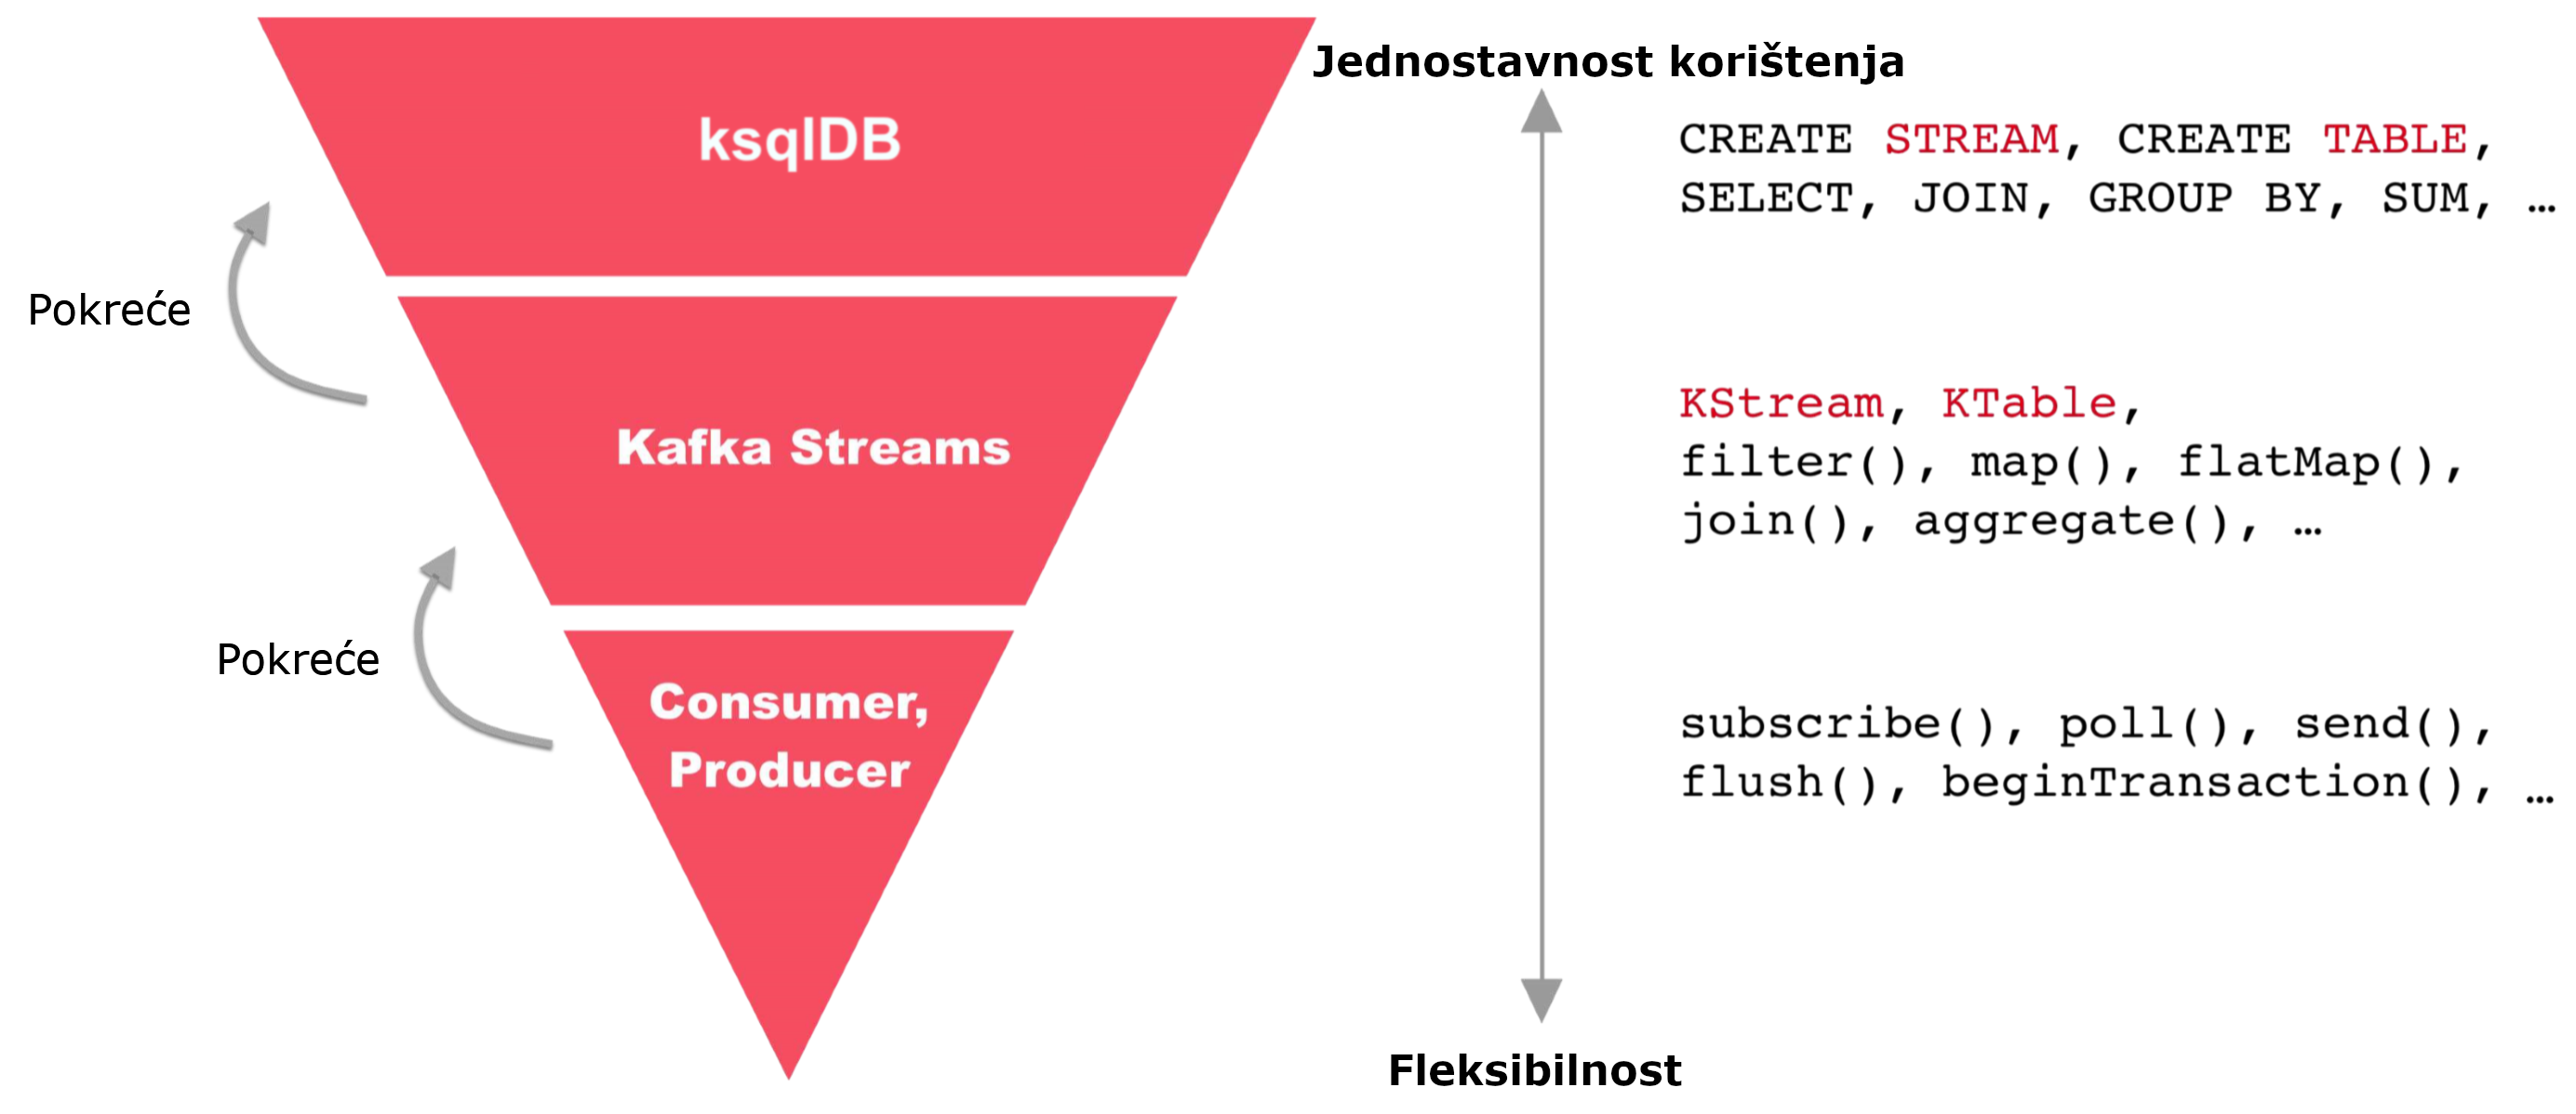
\includegraphics[width=13cm]{images/ksql_streams_consumer.png}
\caption[Hijerarhija Kafka alata]{Hijerarhija Kafka alata\\Slika preuzeta sa \url{https://docs.ksqldb.io/en/latest/operate-and-deploy/how-it-works/}}
\label{fig:ksqldb_streams}
\end{figure}

Sve navedene komponente, koje će biti detaljnije objašnjene u nastavku, zajedno čine moćnu, skalabilnu i prilagodljivu platformu za obradu podataka u stvarnom vremenu. Bilo da koristite producente za izravno slanje poruka u Kafka teme, konzumente za preuzimanje i obradu poruka iz tih tema, Kafka Streams za kompleksnu obradu podataka u stvarnom vremenu, ili ksqlDB za obradu podataka koristeći upite slične SQL-u, Apache Kafka nudi sveobuhvatne alate i funkcionalnosti koje su potrebne za izgradnju robusnih i efikasnih aplikacija za obradu podataka. Ova svestranost i fleksibilnost čine Apache Kafka idealnim izborom za različite scenarije obrade podataka, od jednostavnih do izuzetno složenih.

\subsection{Apache Zookeeper}

Apache ZooKeeper je distribuirana usluga za koordinaciju, otvorenog je koda i koriste ju distribuirane aplikacije. Razvijen je od strane Apache Fundacije i prvi puta izdan u 2008. godini.

ZooKeeper se često koristi za održavanje konfiguracija, pružanje distribuiranog sinkroniziranja, praćenje statusa čvorova u klasteru i pružanje grupnih usluga \citep{hunt_zookeeper_nodate}. Primjerice, u slučaju Apache Kafka, ZooKeeper se koristi za upravljanje i koordinirati brokerima i potrošačima.\\

Međutim, Apache Kafka je nedavno (u vrijeme pisanja ovoga rada) prešla sa korištenja ZooKeeper-a na novi protokol konsenzusa nazvan Kafka Raft (Kraft).

Kako \citet{chandrakant_kafkas_2022} navodi, promjena s ZooKeepera na Kraft ima za cilj pojednostaviti arhitekturu Kafke i učiniti je moćnijom. Kraft je varijanta Raft konsenzusnog protokola temeljena na događajima i promjenu koju uvodi smanjuje prozor nedostupnosti kod pogrešaka Kafka Brokera\footnote{Kafka Broker je poslužitelj u distribuiranom sustavu Kafka.} jer može nadoknaditi propuštene događaje iz dnevnika nakon ponovnog pridruživanja. 

-Promjena na Kraft očekuje donijeti značajne koristi zajednici Apache Kafke. Administratori sustava će lakše nadzirati, administrirati i podržavati Kafka, a programeri će se morati nositi s jednostavnijim sigurnosnim modelom za cijeli sustav. Novo upravljanje metapodacima također znatno poboljšava performanse Apache Kafke, omogućujući kontroleru da se brže prebaci na rezervu i obradi mnogo veći broj particija po klasteru.


\clearpage
\subsection{Kafka Streams}
\label{sec:kstream}

Kafka Streams je lagana, ali moćna Java biblioteka za obogaćivanje, transformiranje i obradu tokova podataka u stvarnom vremenu \citep{seymour_mastering_2021}. Ova biblioteka omogućuje obradu događaja \engl{events} iz Kafka tema \engl{topic}, uključujući različite operacije poput agregacija \engl{stream aggregation}, spajanja tokova \engl{stream joining}, filtriranja poruka, itd., koje se zatim nakon definiranih operacija šalju u novu Kafka temu. \\

Kafka Stream pruža jednostavan API za obradu podataka, omogućujući korisnicima da se usredotoče na logiku obrade podataka bez potrebe za upravljanjem infrastrukturom. Jedna od ključnih prednosti Kafka Streams biblioteke je njena sposobnost da obradi podatke u stvarnom vremenu. 
Za razliku od obrade u serijama \engl{batch}, koja obrađuje podatke u određenim vremenskim intervalima, Kafka Streams omogućuje obradu podataka kako oni dolaze, što rezultira nižim latencijama i omogućuje aplikacijama da pruže ažurirane informacije u realnom vremenu \citep{seymour_mastering_2021}.

Kafka Streams također podržava "točno-jednom" \engl{exactly-once} semantiku obrade, što znači da će svaka poruka biti obrađena točno jednom, čime se eliminira mogućnost dvostrukog obrade istih podataka \citep{narkhede_exactly-once_2017}.
Osim toga, Kafka Streams biblioteka je dizajnirana tako da bude lako skalabilna. Aplikacije mogu biti horizontalno skalabilne dodavanjem više instanci aplikacije, a Kafka Streams će automatski uravnotežiti obradu podataka između njih. \\

Jedna od naprednih funkcionalnosti Kafka Streams biblioteke je prozoriranje \engl{windowing}, koje omogućuje obradu podataka unutar određenog vremenskog intervala, poznatog kao prozor. Prozoriranje je posebno korisno kada se podaci trebaju agregirati na temelju vremenskih intervala, kao što su minuta, sat ili dan. Postoje tri glavne vrste prozora u Kafka Streams biblioteci windows čije se karakteristike mogu vidjeti u tablici \ref{tbl:windows}. Ove vrste prozora omogućuju složene analitičke operacije, poput računanja pokretnih prosjeka ili računanja agregata u određenom vremenskom intervalu.

\begin{table}[htb]
\caption{Vrste prozora u Kafka Streams biblioteci}
\label{tbl:windows}
\centering
\begin{tabular}{l|l|r} \toprule
Vrsta prozora & Naziv na engl. & Karakteristika prozora \\ \midrule
Prevrtajući prozor & Tumbling window & Ne preklapa se, imaju veličinu\\
Skakući prozor & Hopping window & Preklapa se, ima veličinu i iznos koliko skače\\
Sjednički prozor & Session window & Određen duljinom neaktivnosti\\
Klizeći prozor & Sliding window & Ima veličinu i klizi \\ \bottomrule
\end{tabular}
\end{table} 

CloudVane trenutno ne koristi biblioteku Kafka Streams za obradu tokova podataka, već se oslanja na ksqlDB servis, koji je detaljno opisan u poglavlju \ref{sec:ksql}. Međutim, za potrebe ovog rada, opisanog u poglavlju \ref{sec:realTimeMonitoring}, kreiran je Kafka Stream koji filtrira i agregira poruke u Kafka temi koristeći prevrtajući prozor.

\clearpage
\subsection{ksqlDB}
\label{sec:ksql}

KsqlDB je specializirana baza podataka za obradu tokova događaja \engl{event streaming database}. Ova platforma značajno pojednostavljuje implementaciju, pokretanje i održavanje aplikacija za obradu tokova podataka integrirajući dvije ključne komponente Kafka ekosustava: Kafka Connect i Kafka Streams \citep{seymour_mastering_2021}.

Kafka Connect, opisan u poglavlju \ref{sec:connect}, je servis koji omogućuje jednostavno povezivanje Kafka s drugim sustavima, bilo da se radi o izvorima podataka za unos u Kafka ili odredištima za izvoz podataka iz Kafka. Integracija Kafka Connecta u ksqlDB omogućuje korisnicima da lako povežu svoje aplikacije s različitim izvorima i odredištima podataka.

Kafka Streams, opisan u poglavlju \ref{sec:kstream}, je biblioteka za obradu podataka koja omogućuje obradu i analizu podataka u stvarnom vremenu. Integracija Kafka Streamsa u ksqlDB omogućuje korisnicima da koriste moćne funkcionalnosti obrade podataka koje Kafka Streams pruža, ali s jednostavnošću upita sličnim SQL-u.

KsqlDB, kombinirajući ove dvije komponente, pruža snažnu platformu za obradu tokova podataka. Korisnici mogu jednostavno implementirati složene obrade podataka koristeći poznati SQL jezik, dok ksqlDB obavlja teški posao povezivanja s izvorima i odredištima podataka i obrade podataka u stvarnom vremenu. Ova integracija omogućuje korisnicima da se usredotoče na logiku svojih aplikacija, umjesto na složenosti upravljanja infrastrukturom obrade podataka. \\

CloudVane se oslanja na ksqlDB klaster za obradu, agregaciju i manipulaciju tokova podataka koje prikuplja od podržanih pružatelja oblaka. ksqlDB ne samo da omogućuje agregaciju podataka, već također provodi filtriranje i transformaciju podataka, pružajući CloudVaneu snažan alat za efikasnu i efektivnu obradu podataka.

\clearpage
\subsection{Kafka Connect}
\label{sec:connect}

Kafka Connect je integralni dio Apache Kafka ekosustava i pruža skalabilan, pouzdan način za kopiranje podataka između Kafka i drugih skladišta podataka \citep{shapira_kafka_2021}.

Kafka Connect je dizajniran da podrži veliki broj izvora \engl{source} i odredišta \engl{sink} podataka, omogućujući korisnicima da jednostavno povežu Kafka s različitim sustavima za skladištenje podataka. To uključuje tradicionalne baze podataka, datotečne sustave, usluge oblaka i mnoge druge.

Jedna od ključnih funkcionalnosti Kafka Connecta je njegova sposobnost da se lako skalira. To znači da može podržati velike količine podataka i veliki broj veza, što ga čini idealnim za velike, podatkovno intenzivne aplikacije.

Uz to, Kafka Connect podržava neke transformacije podataka, omogućujući korisnicima da prilagode podatke kako bi bolje odgovarali njihovim specifičnim potrebama pri ulazu ili izlazu iz Apache Kafke. To može uključivati promjenu formata podataka, dodavanje ili uklanjanje polja, ili nekoliko drugih vrsta manipulacije podacima.

Ukupno gledano, Kafka Connect pruža snažan, fleksibilan način za povezivanje Kafka s različitim skladištima podataka, omogućujući korisnicima da maksimalno iskoriste svoje podatke. \\

U kontekstu CloudVane aplikacije, Kafka Connect se koristi za prijenos podataka koji su agregirani putem ksqlDB-a u ciljnu bazu podataka, konkretno Oracle ATP (Autonomous Transaction Processing) bazu.

Ova funkcionalnost omogućava CloudVaneu da efikasno i pouzdano prenosi obrađene i agregirane podatke iz Kafka ekosustava u Oracle ATP, što dalje omogućava naprednu analizu i obradu tih podataka. Korištenje Kafka Connecta za ovu svrhu osigurava da se podaci prenose na siguran i pouzdan način, uz održavanje visoke razine performansi i skalabilnosti.

Ova integracija između Kafka Connecta, ksqlDB-a i Oracle ATP baze podataka omogućava CloudVaneu da maksimalno iskoristi svoje podatke, pružajući mu snažne alate za obradu podataka u stvarnom vremenu i njihovo pohranjivanje za daljnju analizu i obradu.

\clearpage
\subsection{Avro serializacija i Schema registry}
\label{sec:schema}

Avro je format serijalizacije podataka neovisan od programskom jeziku što omogućuje njegovu široku primjenu u različitim programskim okruženjima \citep{shapira_kafka_2021}. Jedna od ključnih prednosti Avroa je njegova sposobnost smanjenja mrežnog prometa kroz odvajanje sheme podataka od samih vrijednosti i korištenje binarnog formata. Ova značajka omogućuje efikasno upravljanje velikim količinama podataka, što je često ključno u sustavima za obradu podataka u stvarnom vremenu.

Avro također podržava jaku tipizaciju \engl{strong typing}, što znači da svaki podatak ima strogo definiran tip. Ova značajka pomaže u sprječavanju pogrešaka i poboljšava pouzdanost obrade podataka, jer se mogu izbjeći nekompatibilnosti ili nesporazumi oko formata ili strukture podataka.

Za rad s Apache Kafka sustavom, Avro se često koristi u kombinaciji s Apache Schema Registry servisom. Schema Registry je servis koji pomaže u upravljanju shemama i provođenju pravila o shemama, osiguravajući da svi podaci koji se upisuju u Kafka teme prate pre-definiranu shemu. Ovo je ključno za održavanje kompatibilnosti podataka kako se sustav razvija, jer omogućuje promjene u formatu podataka bez gubitka kompatibilnosti s postojećim podacima. \\

Sveukupno, kombinacija Avroa i Schema Registryja pruža robustan okvir za upravljanje i obradu strukturiranih podataka unutar Apache Kafka sustava. Ove tehnologije omogućuju korisnicima da efikasno i pouzdano upravljaju velikim količinama podataka, istovremeno održavajući visoku razinu pouzdanosti i kompatibilnosti. Upravo iz tih razloga, CloudVane aplikacija koristi Avro format za pohranu podataka u Kafka temama i Schema Registry servis za održavanje i upravljanje shemama.

Ova praksa omogućuje CloudVaneu da maksimalno iskoristi prednosti koje Apache Kafka pruža, uključujući skalabilnost, brzinu i pouzdanost. Korištenje Avro formata osigurava da su podaci kompaktni i dobro strukturirani, što poboljšava performanse i omogućuje efikasnu obradu podataka. Istovremeno, upotreba Schema Registry servisa osigurava da su sve sheme podataka dosljedno upravljane i održavane, što pomaže u održavanju kvalitete podataka i kompatibilnosti kroz vrijeme.

\clearpage
\section{Arhitektura aplikacije CloudVane}
\label{sec:architecture}

CloudVane, kako je prethodno navedeno, je distribuirana aplikacija koja se izvodi na Oracle Kubernetes Engine (OKE) platformi. Osim toga, CloudVane je primjer mikroservisne arhitekture, što znači da se sastoji od brojnih servisa, svaki s određenim zadacima unutar cjelokupnog sustava. Ovi servisi su detaljno opisani u tablici \ref{tbl:cloudvaneServices} i \ref{tbl:kafkaServices}, a arhitektura sustava prikazana je na slici \ref{fig:cloudvaneArch}.

Ova struktura omogućuje visoku razinu modularnosti i fleksibilnosti. Svaki servis može se razvijati, skalirati i održavati neovisno o ostalima, što omogućuje brzi razvoj i lako ažuriranje. Također, ova arhitektura omogućuje bolju iskoristivost resursa, jer svaki servis može biti skaliran prema svojim specifičnim potrebama.

U kontekstu CloudVane aplikacije, ova mikroservisna arhitektura omogućuje efikasno upravljanje i obradu velikih količina podataka. Svaki servis može se specijalizirati za određeni aspekt obrade podataka, što rezultira visokom performansom i pouzdanošću cjelokupnog sustava. Detaljan opis svakog CloudVane servisa može se pronaći u tablici \ref{tbl:cloudvaneServices}.

Uzimajući u obzir da CloudVane koristi usluge Apache Kafke, te usluge su smještene u zasebnom Kubernetes prostoru imena\footnote{Kubernetes prostor imena \engl{namespace} je mehanizam za izolaciju resursa klastera.} \engl{namespace} u odnosu na glavne servise CloudVanea. Apache Kafka servisi opisani su u tablici \ref{tbl:kafkaServices}, a protok podataka kroz CloudVane sustav je prikazan na slici \ref{fig:dataCloudvane}.

Ova organizacijska struktura prikazana na slici \ref{fig:cloudvaneArch}, koja uključuje odvajanje produkcijskog klastera od klastera za razvoj i testiranje, omogućuje jasnu segregaciju i izolaciju resursa među različitim komponentama sustava. Takva struktura ne samo da pojačava sigurnost i upravljivost sustava, već i olakšava skaliranje i održavanje svake komponente neovisno jedna o drugoj. Osim toga, ovakva organizacija pruža bolju kontrolu nad resursima te olakšava praćenje i dijagnostiku problema unutar sustava. U konačnici, ovakav pristup omogućuje efikasnije upravljanje resursima i optimizaciju performansi, čime se poboljšava ukupna pouzdanost i efikasnost CloudVane aplikacije.

\clearpage
\begin{longtblr}[
  	caption = {CloudVane servisi na Kubernetesu},
	label = {tbl:cloudvaneServices},
	]{
	colspec = {X[1,l]|X[1,c]}, 
	rowhead = 1,
	}
	\hline
	Naziv servisa & Opis servisa \\
	\hline
	CloudVane Actioner & Upravlja akcijama na oblaku\\
	CloudVane API & REST poslužitelj i autorizacija\\
	CloudVane Back & Spring poslužiteljske strane\\
	CloudVane Chargeback & Omogućuje izradu izvještaja o potrošnji\\
	CloudVane Config & Spring Config server\\
	CloudVane Datacollector Kafka & Dohvaća podatke iz oblaka, obrađuje ih i prosljeđuje u Apache Kafku\\
	CloudVane Datacollector & Dohvaća podatke iz oblaka, obrađuje ih i pohranjuje direktno u bazu podataka\\
	CloudVane Front & Angular poslužitelj klijentske strane \\
	CloudVane Predictioner API & REST poslužitelj predikcijskog sustava\\
	CloudVane Predicioner Worker & Sustav umjetne inteligencije koji računa predikcije\\
	CloudVane Scheduler & Rasporeditelj zadataka CloudVanea\\
	CloudVane User Management & Sustav za upravljanje korisnicima i pravima na platformi \\
	CloudVane Vault & Sustav za sigurnu pohranu korisničkih kredencijala \\
	\hline

\end{longtblr}

\begin{longtblr}[
	caption = {Kafka servisi na Kubernetesu},
	label = {tbl:kafkaServices},
	]{
		colspec = {X[1,l]|X[1,c]}, 
		rowhead = 1,
	}
	\hline
	Naziv Kafka servisa & Opis servisa \\
	\hline
	Kafka Broker & Poslužuje Apache Kafku\\
	Kafka Connect klaster & Upis tokova u bazu podataka\\
	ksqlDB & Obrađuje tokove podataka\\
	Schema Registry & Upravlja shemama podataka
	\hline
	
\end{longtblr}

\clearpage
\begin{figure}[htb]
	\centering
	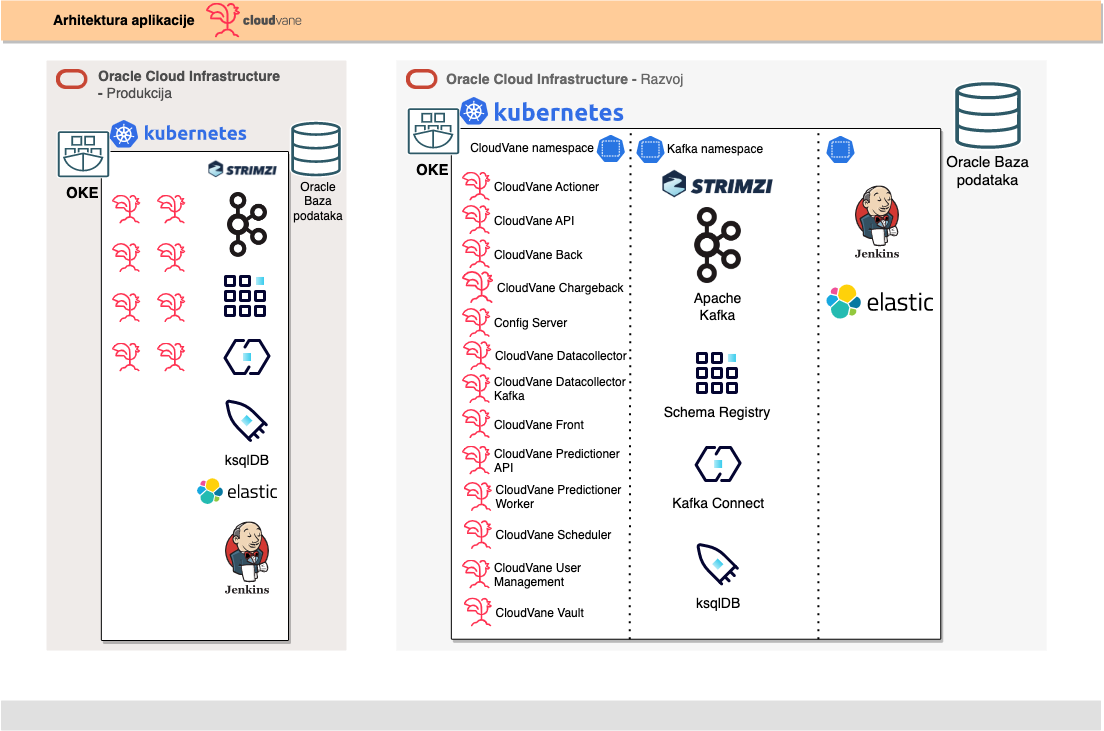
\includegraphics[width=15cm]{images/CloudVaneArchitecture.png}
	\caption[Arhitektura CloudVane sustava]{Arhitektura CloudVane sustava}
	\label{fig:cloudvaneArch}
\end{figure}

\begin{figure}[htb]
	\centering
	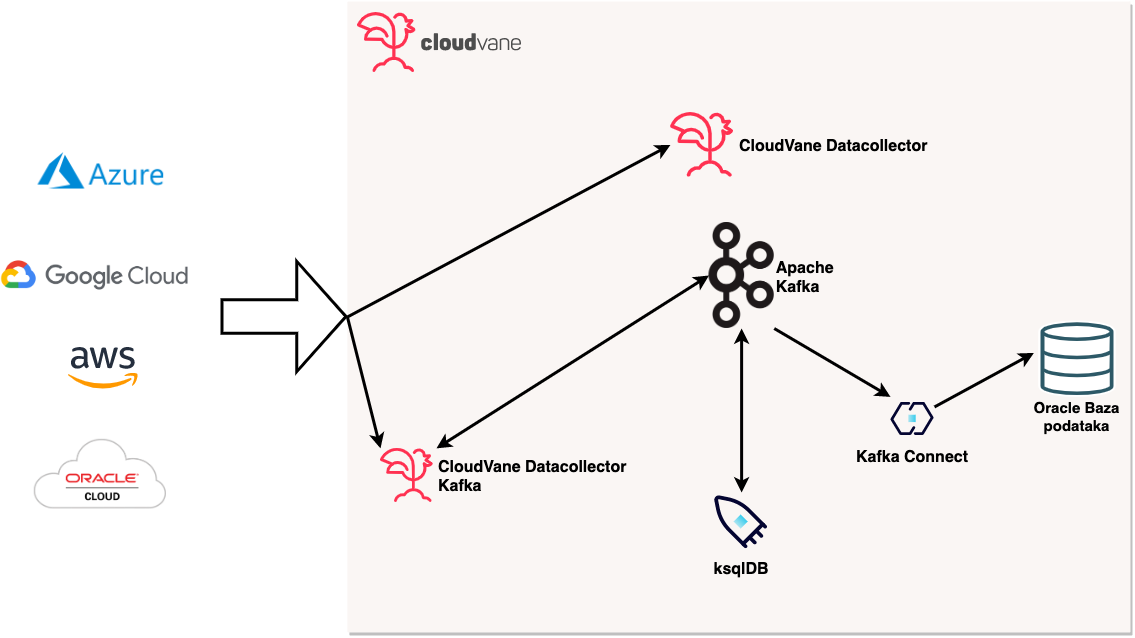
\includegraphics[width=15cm]{images/CloudVaneData.png}
	\caption[Tok podataka CloudVane sustava]{Tok podataka \engl{data pipeline} CloudVane sustava}
	\label{fig:dataCloudvane}
\end{figure}

U kontekstu ovog istraživanja, svi dnevnički zapisi prethodno opisanih servisa, detaljno pojašnjeni u poglavlju \ref{sec:logs}, bit će preusmjereni iz CloudVane klastera u Apache Kafku, smještenu na lokalnom Minikube klasteru. Ova će organizacija omogućiti učinkovitu obradu zapisa te njihovu upotrebu za generiranje rezultata ovoga rada.

\chapter{Nadziranje aplikacija}

Nadziranje \engl{monitoring}, definirano kao sustavno promatranje i provjera ponašanja i izlaza sustava te njegovih komponenti kroz vrijeme \citep{monitorama_monitorama_2016}, ključni je element upravljanja informatičkim sustavima i aplikacijama. Ova strateška praksa, koja se sastoji od stalnog nadzora i analize, omogućuje održavanje optimalnih performansi, stabilnosti i pouzdanosti digitalnih resursa.

Nadzor aplikacija nije samo proces identifikacije i rješavanja problema. On nudi dragocjene uvide koji omogućuju temeljitiju optimizaciju sustava, poboljšanje korisničkog iskustva i osiguranje da sve digitalne komponente funkcionalno integriraju. Sastoji se od kontinuirane provjere, identifikacije anomalija i promptnog rješavanja problema prije nego što se pretvore u kritične situacije. Kroz ovaj proaktivni pristup, nadzor postaje ključan instrument za održavanje visoke razine usluge i postizanje operativne izvrsnosti.\\

U ovom poglavlju rada detaljno se istražuje nadzor distribuirane aplikacije CloudVane, koja je opisana u poglavlju \ref{sec:cloudvane}, s posebnim naglaskom na kontekst dnevničkih zapisa prikazanih u poglavlju \ref{sec:logs}. Upotrebom ELK-a, čije su komponente i funkcionalnosti predstavljene u poglavlju \ref{sec:elk}, ilustrirat će se korištenje sofisticiranih alata za izdvajanje dnevničkih zapisa iz distribuiranih aplikacija unutar Kubernetes grozda. Detaljno će se obraditi procesi prikaza, transformacije i unosa dvnevničkih zapisa u Apache Kafku. Naposljetku, u završnom poglavlju \ref{sec:streamingMonitoring} rad će se fokusirati na nadzor u stvarnom vremenu, pružajući cjelovit prikaz ovog kompleksnog, ali ključnog aspekta upravljanja modernim računalnim sustavima.

\clearpage
\section{Dnevnički zapisi}
\label{sec:logs}

Dnevnički zapisi aplikacija \engl{application logs} ključna su komponenta koja pruža detaljan uvid u rad aplikacije i ključni su za otkrivanje i rješavanje problema, ali i za optimizaciju performansi aplikacije.

Dnevnički zapisi aplikacija sastoje se od sekvencijalno zapisanih događaja koji se događaju unutar aplikacije. Ti događaji mogu biti različite vrste, uključujući informacije o radnji koju je korisnik poduzeo, statusu aplikacije, greškama, upozorenjima i drugim relevantnim informacijama. Dnevnički zapisi pružaju sveobuhvatnu sliku o tome što se događa unutar aplikacije u svakom trenutku.

U kontekstu mikroservisnih arhitektura, kao što je to slučaj s CloudVane aplikacijom, dnevnički zapisi su posebno važni. Budući da je svaki mikroservis odgovoran za svoj dio funkcionalnosti, dnevnički zapisi svakog mikroservisa pružaju uvid u njegov rad. Ako dođe do problema, dnevnički zapisi mogu pomoći u identificiranju koja je komponenta uzrokovala problem.

Međutim, upravljanje dnevničkim zapisima u mikroservisnom okruženju može biti izazovno.. Jedan od najizraženijih je problem agregiranja i pretraživanja dnevničkih zapisa. S obzirom na to da je aplikacija raspoređena na više čvorova unutar Kubernetes grozda, logički i fizički izolirani, konzolidacija i pretraživanje informacija postaje kompleksan zadatak \citep{newman_building_2015}.

U takvom distribuiranom okruženju, svaka komponenta ili mikroservis generira svoje dnevničke zapise. S obzirom na to da su ovi dnevnički zapisi disperzirani preko različitih čvorova, njihova centralizacija zahtijeva robusna i skalabilna rješenja. Bez odgovarajućih alata i strategija, pretraživanje tih zapisa na jednom mjestu može biti prilično izazovno i vremenski zahtjevno. Osim toga, pitanje je i kako oblikovati i strukturirati te zapise na način da pružaju korisne informacije. Različiti mikroservisi mogu imati različite strukture dnevničkih zapisa. Zahtijeva se strategija koja ne samo da agregira ove zapise, već ih i standardizira i strukturira za laku analizu i dijagnostiku. \\

U nastavku poglavlja, fokus će se postaviti na dnevničke zapise programskog jezika Java, što je tematika poglavlja \ref{sec:java}. Fokus na programski jezik Javu proizlazi iz činjenice da je većina servisa unutar distribuirane aplikacije CloudVane upravno razvijena ovim programskim jezikom. Iako i drugi programski jezici nude slične alate za konfiguraciju i upravljanje dnevničkim zapisima, specifičnosti Jave u ovom kontekstu su od posebne važnosti zbog potrebnih konfiguracija. Također, posvetiti će se pažnja ELK alatima, što je centralna tema poglavlja \ref{sec:elk}. Ova dva aspekta čine ključne komponente istraživanja i analize nadzora aplikacija unutar distribuiranih sustava.


\subsection{Dnevnički zapisi u programskom jeziku Java}
\label{sec:java}

CloudVane koristi Logback biblioteku za svoje dnevničke potrebe, koristeći SLF4J apstrakciju. Logback je konfiguriran da ispisuje dnevničke zapise u JSON formatu, što olakšava njihovu obradu, posebno u distribuiranom sustavu gdje različite usluge generiraju zapise. Primjer konfiguracije Logbacka prikazan je u isječku \ref{lst:logback_xml}.

JSON (JavaScript Object Notation) je format koji je lagan za čitanje i pisanje za ljude, a jednostavan za strojeve za obradu. Korištenje JSON formata omogućuje lakšu analizu i obradu dnevničkih zapisa.

Primjer jednog dnevničkog zapisa prikazan je u isječku \ref{lst:cloudvaneLog}. Ovaj zapis ilustrira kako se informacije strukturiraju u JSON formatu.

Osim Logbacka, postoji i Log4j biblioteka, koja je također popularna opcija za dnevničke zapise u Java aplikacijama. Međutim, u kontekstu CloudVane aplikacije, Logback je odabran zbog svoje snažne integracije s SLF4J apstrakcijom i fleksibilnosti u konfiguraciji.


\section{Elastic, Logstash i Kibana (ELK)}
\label{sec:elk}

ELK Stack, akronim koji označava ElasticSearch, Logstash i Kibana, predstavlja snažan skup alata sposoban za prikupljanje, pohranu, analizu i vizualizaciju podataka u realnom vremenu. Najčešće se koristi za upravljanje logovima i praćenje događaja, što ga čini nezamjenjivim alatom za sigurnosne analize, poslovnu inteligenciju i efikasno pretraživanje podataka.. 

U ovom poglavlju se detaljno razmatraju funkcionalnosti svake pojedinačne komponente ELK Stacka, te se demonstrira proces njegove implementacije na lokalni Minikube Kubernetes grozd. Svrha ovog koraka je prilagodba sustava specifičnim potrebama projekta. Arhitektura integriranog sustava prikazana je na dijagramu \ref{fig:archDiagram}, dok je dijagram podataka prikazan na \ref{fig:dataDiagram}.


\subsection{Elastic}
\label{sec:elastic}

Elasticsearch je distribuirani sustav za pretragu i analizu podataka u stvarnom vremenu. Omogućava istraživanje podataka na brz i skalabilan način koji do sada nije bio ostvariv. Koristi se za pretragu cijelog teksta, strukturiranu pretragu, analitiku i kombinaciju sve tri funkcionalnosti \citep{gormley_elasticsearch_2015}.

Zasnovan na Apache Luceneu\footnote{Apache Lucene je snažan sustav za pretraživanje teksta otvorenog koda koji se koristi u brojnim aplikacijama za pretragu i analizu podataka.}, Elasticsearch pruža distribuirani sustav za pretragu teksta s HTTP sučeljem. Ovo sučelje omogućuje jednostavan pristup i manipulaciju podacima kroz standardizirane HTTP protokole. \\

U okviru ELK Stacka, Elasticsearch igra ključnu ulogu kao središnje mjesto za pohranu svih podataka. U ovom slučaju, to su dnevnički zapisi prikupljeni pomoću Logstasha, komponente koja je zadužena za prikupljanje, transformaciju i slanje podataka u Elasticsearch. Logstash je detaljno opisan u poglavlju \ref{sec:logstash}.\\

Elasticsearch ne samo da omogućava pohranu podataka, već nudi i mogućnosti za njihovu detaljnu analizu i pretragu. Ove mogućnosti, u kombinaciji s skalabilnošću i brzinom koju pruža, čine Elasticsearch idealnim izborom za upravljanje velikim količinama podataka u stvarnom vremenu \engl{real-time}.

\subsection{Logstash}
\label{sec:logstash}

Logstash je otvorenog koda i predstavlja moćan sustav za obradu podataka. Njegova glavna svrha je izvlačenje podataka iz različitih izvora, njihova transformacija i obogaćivanje te naknadno slanje prema odredištu \citep{konda_elasticsearch_2023}. Zahvaljujući svojoj arhitekturi baziranoj na tokovima podataka, svaki događaj koji prolazi kroz Logstash obrađuje se prema unaprijed konfiguriranim pravilima. Time se postiže kontinuirana obrada podataka u stvarnom vremenu.\\

U kontekstu ovog rada, Logstash ima ključnu ulogu u prikupljanju dnevničkih zapisa iz nekoliko Apache Kafka tema \engl{topic} te njihovom unosu u Elasticsearch indeks. Konfiguracija je prikazana u isječku koda \ref{lst:logstash}. 

Indeks u Elasticsearch kontekstu je osnovna jedinica za pretragu. Predstavlja kolekciju dokumenata koji imaju slične karakteristike. Indeks je identificiran svojim jedinstvenim imenom, koje se koristi prilikom izvršavanja operacija pretrage, ažuriranja, brisanja i indeksiranja na dokumentima. U ovom radu, indeks se koristi za organiziranje i skladištenje dnevničkih zapisa, omogućavajući njihovu brzu i efikasnu pretragu.

\subsection{Kibana}
\label{sec:kibana}

\citet{gormley_elasticsearch_2015} navode da je Kibana višenamjenska web konzola koja nudi niz opcija, od izvršavanja upita do razvoja nadzornih ploča, grafova i vizualizacija dijagrama za detaljnu analizu i agregacije. Međutim, za komunikaciju s Elasticsearch-om i pozivanje API-ja nije nužno koristiti Kibanu. Na primjer, API-je možemo pozivati koristeći cURL, Postman ili klijente izvornog jezika.\\

Kibana, kao alat za vizualizaciju i istraživanje podataka, u ovom radu koristi se kao sučelje na kojem se mogu kreirati intuitivni grafikoni i izvješća. Ovi elementi omogućuju interaktivno navigiranje kroz velike količine dnevničkih zapisa. S Kibanom je moguće konfigurirati nadzorne ploče koje pružaju vizualne sažetke podataka i omogućuju detaljno istraživanje specifičnih događaja. Primjer prikaza alata Kibane s dnevničkim zapisima može se vidjeti na slici \ref{fig:kibana}.\\

Kibana pruža mogućnost vizualizacije podataka pohranjenih u Elasticsearchu koristeći njene snažne mogućnosti upita i filtriranja. Time se omogućuje detaljna analiza specifičnih metrika ili trendova. Ova funkcionalnost je ključna za učinkovito analiziranje i razumijevanje obimnih podatkovnih setova, kao što su dnevnički zapisi koje obrađuje ovaj rad.

\subsection{Filebeat}
\label{sec:filebeat}

Filebeat je alat za prikupljanje podataka čiji je glavni zadatak skupljanje i centralizacija dnevničkih zapisa. Njegova uloga u ELK Stacku je da nadzire specifične datoteke s dnevničkim zapisima, prikuplja ih i zatim prosljeđuje izravno u Elasticsearch indeks ili Logstash za daljnju obradu. Filebeat je samo jedan od mnogih alata u sklopu Beats platforme\footnote{Beats je platforma koja se sastoji od niza alata za prikupljanje podataka, uključujući dnevničke zapise, mrežni promet, metrike i slično. Svi alati unutar Beats platforme razvijeni su s ciljem jednostavnosti i učinkovitosti.}, koju je razvila tvrtka Elastic. Zbog svog dizajna koji naglašava jednostavnost i minimalnu potrošnju resursa, Filebeat je iznimno pogodan za distribuirane okoline poput Kubernetesa.\\

Iako Logstash nudi moćne mogućnosti obrade podataka, Filebeat je specijaliziran za biti lagan i brz, s naglaskom na efikasno prikupljanje dnevničkih zapisa i njihovo brzo prosljeđivanje do odredišta. To znači da se Filebeat može pokrenuti bez da se to značajno odrazi na performanse. Filebeat i Logstash često se koriste u tandemu; Filebeat je odgovoran za prikupljanje i prosljeđivanje dnevničkih zapisa, a Logstash ih zatim obrađuje i obogaćuje prije konačnog indeksiranja u Elasticsearchu.\\

U okviru ovog rada, Filebeat je implementiran na CloudVane Kubernetes klasteru te je konfiguriran da prikuplja logove s CloudVane servisa. Nakon prikupljanja, ti se logovi prosljeđuju preko interneta na lokalni Minikube Kubernetes klaster, točnije u specifične Apache Kafka teme. Detalji ove konfiguracije prikazani su u isječku koda \ref{lst:filebeat}.

\subsection{Implementacija ELK-a na Kubernetes grozdu}
\label{sec:elk_impl}

U ovom radu, ElasticSearch, Kibana i Logstash implementirani su u lokalnom Kubernetes klasteru koristeći Elasticove prilagođene resurse \engl{Custom Resource Definitions} - CRD\footnote{CRDovi pružaju snažan okvir za stvaranje i upravljanje prilagođenim resursima, omogućujući korisnicima da stvore nove vrste resursa koje se mogu koristiti kao izvorni.}.

Elastic, tvrtka koja razvija ElasticSearch, Kibana i Logstash, pruža skup CRDova za te aplikacije. Ovi CRDovi omogućuju korisnicima da jednostavno implementiraju i upravljaju tim aplikacijama u Kubernetes okruženju, pružajući integrirane mogućnosti za konfiguraciju, skaliranje, sigurnost i monitoriranje.

U kontekstu ovog rada, koristeći Elasticove CRDove, ElasticSearch, Kibana i Logstash pokrenuti su kao zasebni kontejneri unutar Kubernetes klastera. Svaki od ovih kontejnera može se skalirati neovisno, omogućujući fleksibilnu i robusnu infrastrukturu za rad s podacima.

\chapter{Nadziranje stanja distribuiranog sustava u stvarnom vremenu}
\label{sec:streamingMonitoring}

Placeholder

\chapter{Zaključak}
Zaključak.

\bibliography{literatura}
\bibliographystyle{fer}


\lstset{
	aboveskip=3mm,
	belowskip=3mm,
	showstringspaces=false,
	columns=flexible,
	basicstyle={\small\ttfamily},
	numbers=none,
	numberstyle=\tiny\color{gray},
	keywordstyle=\color{blue},
	commentstyle=\color{dkgreen},
	stringstyle=\color{mauve},
	breaklines=true,
	breakatwhitespace=true,
	tabsize=3
}


\appendix
\chapter{Isječci programskog koda}
\label{sec:code}


\begin{lstlisting}[caption={Primjer dnevničkog zapisa CloudVane servisa}
		,label={lst:cloudvaneLog}
		,language=json]
{
	"@timestamp": "2023-06-11T20:32:51.032Z",
	"@version": "1",
	"message": "Calling data_collector.prepare_cost_history for cloud account id: 76.",
	"logger_name": "hr.neos.cloudvane.datacollector.predictioner. PredictionerService",
	"thread_name": "scheduling-1",
	"level": "INFO",
	"level_value": 20000
}
\end{lstlisting}

\clearpage
\begin{lstlisting}[caption={Konfiguracija Logback-a}
	,label={lst:logback_xml}
	,language=XML]
<?xml version="1.0" encoding="UTF-8"?>
<configuration>
<contextName>cloudvane-dc-kafka</contextName>

<!-- Include CONSOLE_LOG_PATTERN -->
<include resource="org/springframework/boot/logging/logback/defaults.xml"/>

<appender name="CONSOLE_PATTERN" class="ch.qos.logback.core.ConsoleAppender">
<layout class="ch.qos.logback.classic.PatternLayout">
<Pattern>${CONSOLE_LOG_PATTERN}</Pattern>
</layout>
</appender>

<appender name="CONSOLE_JSON" class="ch.qos.logback.core.ConsoleAppender">
<encoder class="net.logstash.logback.encoder.LogstashEncoder" />
</appender>

<springProfile name="local">
<root level="INFO">
<appender-ref ref="CONSOLE_PATTERN" />
</root>
</springProfile>

<springProfile name="dev,dev-test,test,prod">
<root level="INFO">
<appender-ref ref="CONSOLE_JSON" />
</root>
</springProfile>
</configuration>
\end{lstlisting}

\clearpage
\begin{lstlisting}[caption={Primjer dnevničkog zapisa sa CloudVane servisa sa metapodacima}
		,label={lst:cloudvaneLog}
		,language=json]
{
	"@timestamp": "2023-05-03T17:00:04.068Z",
	"@metadata": {
		"beat": "filebeat",
		"type": "_doc",
		"version": "8.7.1"
	},
	"log": {
		"offset": 294991,
		"file": {
			"path": "/var/log/containers/cloudvane-datacollector..."
		}
	},
	"level_value": 20000,
	"logger_name": "hr.neos.cloudvane.datacollector.collector.cloud.azure.
	AzureCollectionService",
	"ecs": {
		"version": "8.0.0"
	},
	"host": {
		"ip": [
		"10.244.1.90",
		"fe80::8bf:80ff:fe5f:3832"
		],
		"mac": [
		"0A-BF-80-5F-38-32"
		],
		"hostname": "filebeat-kafka-matej-44gl2",
		"architecture": "x86_64",
		"os": {},
		"containerized": true,
		"name": "filebeat-kafka-matej-44gl2"
	},
	"stream": "stdout",
	"input": {
		"type": "container"
	},
	"instana.trace.id": "adf2108f84007f73",
	"level": "INFO",
	"container": {
		"id": "a248de8e52ca95d0591cd220cd4f
		438488e4765bc1de51644c4c7621784b9e45",
		"runtime": "cri-o",
		"image": {
			"name": "fra.ocir.io/frpf7jvyycgx/cv-kafka/openjdk-17/
			cloudvane-datacollector:1fc43..."
		}
	},
	"message": "Fetching AZURE cost file list from URL: 
	https://storageaccounttestcv.blob.core.windows.net/
	dailycontainer?restype=container&comp=list",
	"agent": {
		"ephemeral_id": "5c71c9f5-3073-4b71-90a8-04ef13492db4",
		"id": "18a62338-ce41-4a14-9d6d-e9f6887041b0",
		"name": "filebeat-kafka-matej-44gl2",
		"type": "filebeat",
		"version": "8.7.1"
	},
	"@version": "1",
	"thread_name": "scheduling-1",
	"kubernetes": {
		"labels": {
			"app": "cloudvane-datacollector-kafka",
			"client": "test",
			"pod-template-hash": "75f86b6d7c"
		},
		"container": {
			"name": "cloudvane-datacollector"
		},
		"node": {
			"labels": {	},
			"hostname": "10.38.1.11",
			"name": "10.38.1.11",
			"uid": "9c999e81-cafc-405c-936c-8c45183351b5"
		},
		"pod": {
			"ip": "10.244.1.5",
			"name": "cloudvane-datacollector-kafka-test-75f86b6d7c-g2kgb",
			"uid": "1a2ff384-ac41-47d0-815d-43c27591cff7"
		},
		"namespace": "cloudvane-test",
		"namespace_uid": "4af72ed8-18a8-4d35-ad03-966d1804e9c7",
		"namespace_labels": {
			"kubernetes_io/metadata_name": "cloudvane-test"
		},
		"replicaset": {
			"name": "cloudvane-datacollector-kafka-test-75f86b6d7c"
		}
	},
	"indexName": "cloudvane-datacollector-kafka"
}
\end{lstlisting}

\clearpage
\begin{lstlisting}[caption={Konfiguacija Logstasha na lokalnom Kubernetes grozdu}
	,label={lst:logstash}]
input {
	kafka {
		bootstrap_servers => "masters-cluster-kafka-bootstrap.kafka.svc.cluster.local:9092"
		topics_pattern => "^logs.*"
		group_id => "logstash"
		codec => "json"
		decorate_events => "extended"
	}
}
filter {
	mutate {
		add_field => { "topic" => "%{[@metadata][kafka][topic]}" }
	}
}
output {
	elasticsearch {
		
		hosts => ["https://masters-es-internal-http.elk.svc.cluster.local:9200"]
		index => "k8s-%{topic}"
		
		ssl => true
		ssl_certificate_verification => false
		user => "elastic"
		password => "ELASTIC_PASSWORD"
		
		ilm_enabled => false
	}
}
\end{lstlisting}

\clearpage
\begin{lstlisting}[caption={Konfiguacija Filebeata na CloudVane Kubernetes grozdu}
	,label={lst:filebeat}
	,language=yaml]
filebeat.inputs:
- type: container
format: cri
paths:
- /var/log/containers/*.log
processors:
- decode_json_fields:
fields: [ "message" ]
target: ""
overwrite_keys: true
- add_kubernetes_metadata:
in_cluster: true
host: ${NODE_NAME}
matchers:
- logs_path:
logs_path: /var/log/containers/
- script:
lang: javascript
source: >
function process(event) {
	var appName=event.Get("kubernetes.labels.app");
	if (appName!==null && appName.indexOf("cloudvane") !== -1)
	{
		event.Put("indexName",event.Get("kubernetes.labels.app"));
	}
	else if (appName!==null && appName.indexOf("kafka")!== -1)
	{
		event.Put("indexName","cloudvane-".concat(event.Get("kubernetes.labels.app")));
	}
	else
	{
		event.Put("indexName","other");
	}
	var input = event.Get("message");
	input = input.replace(/RequestId:[^ ]*/g, "");
	input = input.replace(/Time:[^ ]*/g, "");
	input = input.replace(/\d{4}-\d{2}-\d{2} \d{2}:\d{2}:\d{2}\.\d{3}/g, "");
	input = input.replace(/\d{4}-\d{2}-\d{2} \d{2}:\d{2}:\d{2},\d{3}/g, "");
	var kafkaKey = {
		"message": input,
		"service": event.Get("indexName"),
		"kubernetes": {
			"namespace": event.Get("kubernetes.namespace"),
			"pod": event.Get("kubernetes.pod.name")
		}
	};
	event.Put("kafkaKey", JSON.stringify(kafkaKey));
}    
- drop_event:
when:
not:
or:
- equals:
kubernetes.namespace: "cloudvane-test"
- equals:
kubernetes.namespace: "kafka-test"
- type: log
paths:
- /var/log/containers/*.out
processors:
- decode_json_fields:
fields: [ "message" ]
target: ""
overwrite_keys: true
- script:
lang: javascript
source: >
function process(event) {
	event.Put("indexName","usage");
	var kafkaKey = {
		"message": event.Get("message"),
		"service": event.Get("indexName"),
	};
	event.Put("kafkaKey", JSON.stringify(kafkaKey));
}
processors:
- add_host_metadata:
setup.template:
name: k8s
pattern: k8s-*
setup.ilm.enabled: false
output.kafka:
hosts: [ "MY_PUBLIC_IP:30096" ]
version: '2.6.0'
key: '%{[kafkaKey]}'
topic: 'logs-%{[indexName]}-%{[kubernetes.namespace]}'
partition.round_robin:
reachable_only: false
required_acks: 1
batch.max_events: 2048
compression: snappy
max_message_bytes: 1000000
ssl.enabled: true
ssl.certificate_authorities: [ '/etc/filebeat/ssl/ca.pem' ]
ssl.certificate: '/etc/filebeat/ssl/certificate.pem'
ssl.key: '/etc/filebeat/ssl/key.pem'
\end{lstlisting}


\begin{sazetak}
Sažetak na hrvatskom jeziku.

\kljucnerijeci{Kubernetees, Apache Kafka, Tokovi Podataka, Dnevnički zapisi, Obrada u stvarnom vremenu, Elastic, ELK, Nadzor aplikacija, Grozd računala}
\end{sazetak}

\engtitle{Real-Time Log Analysis for Monitoring Distributed Systems}
\begin{abstract}
Abstract.

\keywords{Kubernetes, Apache Kafka, Streaming, Real-Time, Logs, Elastic, ELK, Monitoring, Cluster}
\end{abstract} 

\end{document}
